% !TEX program = pdflatex
% Standard IEEE Transactions journal format.
\documentclass[journal]{IEEEtran}

\usepackage{amsmath,amssymb,amsfonts}
\usepackage{bm}
\usepackage{mathtools}
\usepackage{graphicx}
\usepackage{booktabs}
\usepackage{array}
\usepackage{multirow}
\usepackage{placeins}
\usepackage{xcolor}
\usepackage{tikz}
\usetikzlibrary{arrows.meta,positioning,calc,fit,matrix,shapes.geometric}
\usepackage{url}
\usepackage{cite}
\usepackage[nameinlink,capitalize]{cleveref}

\graphicspath{{figures/}}

\newcommand{\SMPCC}{S-MPCC}
\newcommand{\MPCC}{MPCC}
\newcommand{\MPC}{MPC}
\newcommand{\MpcLocalPlanner}{MPC local planner}

\newcommand{\vx}{\bm{x}}
\newcommand{\vu}{\bm{u}}
\newcommand{\vp}{\bm{p}}
\newcommand{\vr}{\bm{r}}
\newcommand{\xr}{\bm{x}_{r}}
\newcommand{\xl}{\bm{x}_{\ell}}
\newcommand{\xaug}{\bm{x}}
\newcommand{\ec}{e_{\mathrm{c}}}
\newcommand{\el}{e_{\mathrm{l}}}
\newcommand{\dd}{\mathrm{d}}
\newcommand{\R}{\mathbb{R}}
\newcommand{\Pending}{\textcolor{spmpcgray}{\textit{pending}}}
\newcommand{\PendingResult}[1]{%
  \par\smallskip\noindent
  \textcolor{spmpcgray}{\textit{Pending result: #1}}%
  \par\smallskip}

\definecolor{spmpcblue}{RGB}{36,99,180}
\definecolor{spmpclight}{RGB}{235,243,255}
\definecolor{spmpcorange}{RGB}{220,120,40}
\definecolor{spmpcgray}{RGB}{90,90,90}

\title{\SMPCC: Slosh-Aware Model Predictive Contouring Control for Open-Liquid Transport on Mobile Bases}

\author{Renjun Zhang%
\thanks{Renjun Zhang is with the University of Science and Technology of China,
Hefei, China (e-mail: zhangrenjun@mail.ustc.edu.cn).}}

\begin{document}

\maketitle

\begin{abstract}
Transporting an open liquid on a mobile base requires more than suppressing command variation: the response to a candidate motion also depends on the liquid displacement, velocity, and oscillation phase already present when that motion is planned.
This paper presents an online receding-horizon local motion planner and controller for a prescribed geometrically feasible path.
The proposed \SMPCC{} formulation jointly predicts robot motion, virtual path progress, and a container-parameterized first lateral sloshing mode represented in two orthogonal directions.
An odometry-driven propagation step carries the modal state between control cycles, so the current liquid dynamic memory can alter the next optimized motion segment.
The frozen evaluation protocol uses matched slosh-agnostic and smooth-only MPCC variants, an independently tuned completion-time-matched comparison, geometry-based transfer without controller-weight retuning, controlled liquid-phase studies, counterfactual replay of the propagated runtime state, and command-chain and runtime audits.
The scope is online motion generation along a supplied path; global route planning, obstacle reasoning, and a formal spill-free guarantee are not claimed.
\end{abstract}

\begin{IEEEkeywords}
mobile robots, open-liquid transport, liquid sloshing, model predictive contouring control, receding-horizon planning
\end{IEEEkeywords}

% \section{Introduction}

Mobile robots are increasingly deployed in indoor laboratory, service, and industrial transport scenarios.
A representative task is the transportation of open or partially open liquid containers.
Unlike rigid payloads, the liquid free surface can oscillate under base acceleration, braking, and turning.
For liquid transport, such oscillations can reduce task efficiency, cause sample loss or environmental contamination, introduce additional settling time, and eventually lead to task failure.
Consequently, effective base motion must be not only geometrically feasible and smooth, but also informed by the dynamic response of the transported liquid.

This paper considers the following problem: given a geometrically feasible reference path, how can a standard wheeled mobile base generate executable online local motion while predicting and reducing the open-liquid response excited by its own motion?
The central premise is that \emph{liquid sloshing is not merely a trajectory-smoothing problem, but a state-prediction problem with dynamic memory}.
Motion sequences with similar velocity, acceleration, or jerk bounds may induce different liquid responses because the future free-surface motion depends on the current modal displacement, modal velocity, and residual oscillation phase.

Prior work has reduced liquid sloshing through low-order modeling, input shaping, velocity-profile design, trajectory optimization, and tracking control \cite{A02_Guagliumi2021,A01_Leva2021,A07_Singer1990,A12_Okatsuka2011,C05_Okatsuka2012}.
In parallel, mobile-robot local planners can generate online commands that satisfy motion constraints, path tracking, and local navigation requirements \cite{D15_Fox1997,D16_Rosmann2017,D17_Rosmann2021,D19_Liniger2015,D20_Brito2019}.
These two lines of work usually do not meet at the same decision layer.
Anti-slosh methods often operate on a prescribed path or trajectory, solve an offline optimization problem, design a velocity profile, or act as a tracking or special-platform controller.
General local planners are online and deployable, but they typically do not propagate the dynamic state of the transported liquid.
This work therefore targets the intersection of these two lines: online local planning for a standard mobile base that must consider path progress, command feasibility, and future liquid response within the same receding-horizon problem.

The resulting planner must address three technical issues.
First, the liquid response is not a static function of the instantaneous acceleration or curvature; a smooth future command sequence can still amplify residual oscillations if it is poorly phased with the current liquid state.
Second, ordinary local planning methods such as DWA, TEB, MPCC, MPPI, and jerk-limited trajectory generation can produce executable robot motion, but their states and objectives generally focus on robot feasibility, path error, obstacle risk, control smoothness, or time efficiency rather than liquid modal variables such as $[\eta,\dot{\eta}]$.
Third, existing anti-slosh methods demonstrate the value of liquid modeling, but many of them are not formulated as an online local planner that repeatedly solves a short-horizon optimal control problem from the current robot, path, and liquid state and outputs standard base velocity commands.

To address this gap, we propose \SPMPC{}, a slosh-aware model predictive contouring control method.
\SPMPC{} uses \MPCC{} as the local-planning backbone and augments the robot and path-progress states with a low-order slosh modal state.
The planner predicts base motion and liquid response over a finite horizon and jointly optimizes path-tracking errors, path progress, executable base control, control smoothness, and predicted slosh response.
In contrast to methods that only penalize velocity, acceleration, or control variation, \SPMPC{} allows the current modal displacement and velocity of the liquid to influence future motion selection.
In contrast to tracking controllers applied after a trajectory is generated, \SPMPC{} incorporates the liquid response at the local trajectory-generation stage.
In contrast to offline global anti-slosh trajectory optimization, it retains the interface and receding-horizon execution pattern of a mobile-robot local planner.

\begin{figure}[t]
  \centering
  \resizebox{\linewidth}{!}{%
  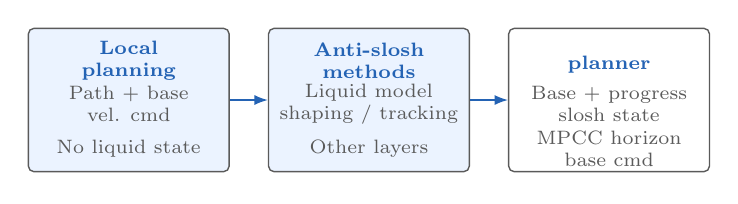
\begin{tikzpicture}[
    font=\footnotesize,
    panel/.style={draw=spmpcgray, rounded corners=2pt, line width=0.5pt, fill=spmpclight, minimum width=2.55cm, minimum height=1.82cm, align=center},
    title/.style={font=\bfseries\scriptsize, text=spmpcblue, align=center},
    note/.style={font=\scriptsize, text=spmpcgray, align=center},
    arr/.style={-{Latex[length=1.7mm]}, line width=0.5pt, draw=spmpcblue}
  ]
    \node[panel] (p1) at (0,0) {};
    \node[title] at (p1.north) [yshift=-0.42cm] {Local\\planning};
    \node[note] at (p1.center) [yshift=-0.05cm] {Path + base\\vel. cmd};
    \node[note] at (p1.south) [yshift=0.30cm] {No liquid state};

    \node[panel] (p2) at (3.05,0) {};
    \node[title] at (p2.north) [yshift=-0.42cm] {Anti-slosh\\methods};
    \node[note] at (p2.center) [yshift=-0.05cm] {Liquid model\\shaping / tracking};
    \node[note] at (p2.south) [yshift=0.30cm] {Other layers};

    \node[panel, fill=white] (p3) at (6.10,0) {};
    \node[title] at (p3.north) [yshift=-0.42cm] {\SPMPC{}\\planner};
    \node[note] at (p3.center) [yshift=-0.05cm] {Base + progress\\slosh state};
    \node[note] at (p3.south) [yshift=0.30cm] {\MPCC{} horizon\\base cmd};

    \draw[arr] (p1.east) -- (p2.west);
    \draw[arr] (p2.east) -- (p3.west);
  \end{tikzpicture}}
  \caption{Positioning of \SPMPC{}. Ordinary local planners provide online mobile-base interfaces but usually do not propagate liquid states; existing anti-slosh methods explicitly model liquid dynamics but often operate at other decision layers. This work embeds a low-order slosh state into an online \MPCC{} local-planning problem for standard mobile bases.}
  \label{fig:system_overview}
\end{figure}

The contributions are summarized as follows.
\begin{enumerate}
  \item \textbf{Dynamic-memory augmented online \MPCC{} local planning.}
  We formulate an online slosh-aware local-planning problem for mobile-base open-liquid transport and construct an \MPCC{} framework that propagates a low-order slosh modal state together with robot motion and path progress.
  The same receding-horizon optimal control problem jointly optimizes path errors, path progress, base-control smoothness, and predicted slosh response.
  \item \textbf{Finite-horizon predictive reference adaptation.}
  We introduce a soft Slosh-risk Reference Governor that evaluates candidate speed-reference scaling factors using short-horizon slosh prediction.
  The governor supplies a conservative speed reference to the \MPCC{} problem without changing its state dimension and without directly overriding the final base command.
  \item \textbf{Evaluation protocol separating model proxies and external liquid observations.}
  We organize internal ablations, ordinary local-planner comparisons, mobile-base anti-slosh references, and model-to-external consistency analysis to evaluate the independent role of explicit slosh-state prediction while avoiding the misinterpretation of internal proxy variables as measured liquid-surface quantities.
\end{enumerate}

The scope of the paper is online slosh-aware local planning along a precomputed geometrically feasible reference path.
The method is not presented as the first slosh-aware \MPC{} formulation, a complete dynamic-obstacle navigation system, a high-fidelity free-surface simulator, a formal spill-free controller, or a closed-loop controller driven by measured free-surface feedback.
Internal slosh-height proxies are used for optimization and diagnosis; claims about real liquid motion rely on external visual or liquid-level observations.
The Slosh-risk Reference Governor is a soft reference-adaptation module, not a hard safety interlock: it modifies the speed reference entering the \MPCC{} problem and does not directly replace the final base command.

% \section{Related Work}

This section organizes related work by both platform proximity and decision-layer proximity.
The paper does not address liquid sloshing in isolation, nor does it address generic mobile-robot local planning in isolation.
Instead, it focuses on their intersection at the online local-planning layer of a standard wheeled mobile base, where the planner must output executable commands at runtime while propagating the dynamic state of the transported liquid over the prediction horizon.

Three groups of prior work are most relevant.
The first group consists of ordinary mobile-robot local planners and trajectory optimization methods, which operate at a similar deployment layer but generally do not propagate liquid states.
The second group includes mobile-base liquid transport and closely related anti-slosh studies, which share the physical task but often operate through fixed paths, velocity profiles, offline trajectory optimization, tracking control, or special platform mechanisms.
The third group covers cross-platform slosh modeling, anti-slosh trajectory generation, and predictive control, which provide modeling and control foundations while clarifying the novelty boundary of this work.

\subsection{Online Local Planning and Trajectory Optimization for Mobile Robots}

Mobile-robot local planners address short-horizon motion generation at runtime and must output executable base commands under kinematic, dynamic, and environmental constraints.
Classical DWA, TEB, and \MpcLocalPlanner{} represent important families of velocity-space search, time-parameterized trajectory optimization, and receding-horizon nonlinear optimal control \cite{D15_Fox1997,D16_Rosmann2017,D17_Rosmann2021}.
\MPCC{} has also become a useful backbone for progress-maximizing path following and local planning \cite{D19_Liniger2015,D20_Brito2019}.
Regulated pure pursuit, dynamic-window variants, LT-DWA, MPPI, differential-drive trajectory optimization, and jerk-limited trajectory generation further extend local planning in terms of tracking, velocity and acceleration limits, dynamic feasibility, risk handling, and smoothness \cite{D01_Macenski2023,D22_Ohnishi2026,D02_Jian2023,D06_Williams2017,D07_Trevisan2025,D03_Zhang2025,D13_Berscheid2021}.

These methods are close to the system interface considered here because they serve runtime local decision making and ultimately produce executable base commands.
Local-planner benchmarks also typically evaluate safety, efficiency, smoothness, path tracking, and computation time \cite{D21_Wen2021}.
They therefore provide decision-layer context for \SMPCC{}, although the current fixed-path study does not rank global or obstacle-oriented planners.

However, these planners usually propagate robot pose, velocity, path error, obstacle distance, control variation, or risk variables; they do not include the modal displacement and velocity of the liquid inside the transported container.
For liquid transport, reducing command variation or improving geometric smoothness is not equivalent to suppressing sloshing.
Two command sequences may have similar velocity, acceleration, and jerk profiles but different future liquid responses because they couple differently with the current liquid phase.
Ordinary local planners clarify the same-layer novelty boundary, but they do not directly represent liquid dynamic memory.

\subsection{Mobile-Base Liquid Transport and Anti-Slosh Methods}

Mobile-base liquid transport is the closest physical task to this paper.
Hamaguchi and collaborators studied path design, velocity profiles, input shaping, and tracking control for wheeled mobile robots or carts transporting cylindrical liquid containers \cite{B04_Hamaguchi2002,B03_Hamaguchi2004,B02_Hamaguchi2005}.
These studies demonstrated that mobile-platform motion excites liquid sloshing and that motion planning and control benefit from explicit consideration of the liquid response.
Subsequent work also introduced active vibration reducers, parallel-link mechanisms, and omnidirectional mobile platforms \cite{B05_Hamaguchi2019,B06_Hamaguchi2018,B07_Nguyen2024,B08_Yuan2020}, showing that anti-slosh transport can be achieved through specialized hardware or platform designs as well as software planning.

Recent work has further incorporated liquid models into mobile-robot or mobile-container optimization and control.
Lim et al.\ approximate liquid sloshing by spherical-pendulum dynamics and solve a two-dimensional trajectory optimization problem to reduce sloshing \cite{B01_Lim2024}.
Nguyen Viet et al.\ combine a nonlinear equivalent mass-spring-damper model, time-optimal planning, tracking control, and output constraints for container transport under disturbances \cite{B11_Viet2025}.
Prabakaran et al.\ study slosh-aware trajectory control and \MPC{} tracking control on a reconfigurable stair-climbing service robot \cite{B12_Prabakaran2026}.

These studies establish the value of explicit liquid modeling and optimized motion generation.
Their main difference from this work is the decision layer.
The Hamaguchi line of work is closer to path design, velocity-profile design, input shaping, and tracking along a prescribed route.
Active suppression mechanisms rely on additional hardware or special platforms.
The approach of Lim et al.\ is closer to whole-trajectory offline optimization.
Nguyen Viet et al.\ use a planning-plus-tracking structure, and Prabakaran et al.\ focus on a special service-robot platform and trajectory tracking.
In contrast, \SMPCC{} inserts a low-order slosh state directly into an online \MPCC{} local-planning problem for a standard wheeled mobile base and resolves a short-horizon optimization problem at every control cycle.

\begin{table}[t]
  \centering
  \scriptsize
  \setlength{\tabcolsep}{3pt}
  \caption{Decision-layer comparison with mobile-base liquid-transport studies.}
  \label{tab:mobile_base_related_work_framework}
  \begin{tabular}{p{0.23\linewidth} p{0.29\linewidth} p{0.36\linewidth}}
    \toprule
    Type & Representative work & Main difference from this paper \\
    \midrule
    Fixed path, velocity profile, and input shaping & Hamaguchi series \cite{B04_Hamaguchi2002,B03_Hamaguchi2004,B02_Hamaguchi2005} & Suppresses sloshing mainly through predesigned paths or speed profiles rather than a path-progress \MPCC{} solved at every control cycle. \\
    Active suppression hardware & Mobile carts or omnidirectional platforms with active reducers \cite{B05_Hamaguchi2019,B06_Hamaguchi2018} & Relies on additional mechanisms or special platforms rather than a software local planner for a standard wheeled base. \\
    Offline liquid-constrained trajectory optimization & Lim et al. \cite{B01_Lim2024} & Uses explicit liquid dynamics but is closer to whole-trajectory optimization than runtime local planning. \\
    Time-optimal planning and tracking control & Nguyen Viet et al. \cite{B11_Viet2025} & Uses reference planning and robust tracking rather than directly producing local-planner base commands. \\
    Slosh-aware tracking on special platforms & Prabakaran et al. \cite{B12_Prabakaran2026} & Demonstrates slosh-aware \MPC{} or tracking control, but with different platform, task interface, and control layer. \\
    \bottomrule
  \end{tabular}
\end{table}

Thus, the mobile-base liquid-transport problem is not unexplored.
The gap addressed here is the insertion of liquid dynamic memory into the online local-planning loop of a standard mobile base.
\SMPCC{} defines this problem layer by selecting path progress, base control, and predicted liquid response in the same receding-horizon optimization problem.

\subsection{Cross-Platform Slosh Modeling, Trajectory Generation, and Predictive Control}

Liquid sloshing also appears in manipulators, SCARA systems, liquid-transfer machines, tank vehicles, ships, and specialized mechanisms.
High-fidelity VOF, FEM, CFD, and digital-twin models can describe complex free-surface behavior, fluid-structure coupling, and nonlinear effects \cite{A03_Schrgenhumer2019,A04_Elahi2015,A05_Nicolsen2017,A06_Moya2020}.
However, their state dimension and computational cost are generally unsuitable for direct embedding in a real-time mobile-robot local planner.
Equivalent-pendulum, mass-spring-damper, and low-order modal models instead provide a compact state representation of dominant slosh dynamics, making them more appropriate as prediction models for online optimization \cite{A02_Guagliumi2021,A01_Leva2021}.

Input shaping, predictive control, and anti-slosh trajectory generation have shown that explicit liquid models can improve motion generation and control \cite{A07_Singer1990,A12_Okatsuka2011,C05_Okatsuka2012,C01_Ferrari2026,C02_Muchacho2022,C03_Moriello2018,C04_Kuriyama2008,C06_Viet2024}.
Ferrari et al.\ propose offline time-optimal anti-slosh trajectory planning for multi-container transport on a 4D SCARA system and compare a low-order model height with video-extracted experimental liquid motion \cite{C01_Ferrari2026}.
That work provides a useful model-to-experiment validation perspective, but differs in platform, grasping configuration, optimization layer, and online interface.
Accordingly, this paper does not claim novelty as the first use of a slosh state in \MPC{}; it emphasizes the integration of a low-order slosh state into the online local-planning layer of a standard mobile base.

External sensing, machine vision, and liquid-level detection studies further show that real liquid motion can be evaluated using independent observations \cite{A08_Weaver2024,A09_Bobovnik2021,A10_Shao2026,A11_Ren2024}.
This motivates the distinction used throughout the paper between internal model proxies and measured liquid-surface indicators.
Cross-platform anti-slosh studies are therefore treated primarily as modeling and evaluation references unless their platform, input interface, and decision layer can be reproduced under the same experimental conditions.

\subsection{Positioning of \SMPCC{}}

In summary, prior work has established foundations in mobile-robot local planning, mobile-base liquid transport, low-order slosh modeling, and anti-slosh predictive control.
Ordinary local planners operate at a similar deployment layer but usually lack liquid-state prediction.
Mobile-base anti-slosh methods share the physical task but often operate through fixed paths, speed profiles, offline optimization, tracking control, or special platforms.
Cross-platform anti-slosh methods provide modeling and control foundations but do not generally constitute same-layer experimental baselines.

This paper is positioned at their intersection: online slosh-aware \MPCC{} local planning for a standard wheeled mobile base.
Rather than claiming the first slosh-aware \MPC{} method, \SMPCC{} integrates low-order slosh modal states, path progress, base-control constraints, control smoothness, and predicted liquid response into one receding-horizon local-planning problem. Its empirical claims remain limited to matched internal \MPCC{} variants, completion-time control, geometry-based container transfer, controlled liquid-phase planning, propagated-state replay, and shared execution-layer and runtime audits.

\section{Problem Formulation and \SPMPC{} Method}

This section presents the \SPMPC{} formulation.
The anti-slosh requirement for open-liquid transport is handled at the online local-planning layer of a standard mobile base.
Given a precomputed geometrically feasible reference path, the planner solves a receding-horizon \MPCC{} problem whose state includes the robot state, path progress, and a low-order slosh state, and outputs executable base velocity commands.
Unlike offline anti-slosh trajectory generation, fixed-path speed profiling, or tracking control after a trajectory has been prescribed, \SPMPC{} replans from the current augmented state at every control cycle.
Unlike smoothness-only planners, it explicitly propagates liquid dynamic memory in the prediction model.
The method does not attempt high-fidelity free-surface simulation; it uses a control-oriented low-order slosh model suitable for online optimization.
On top of the basic planner, we also formulate a finite-horizon reference-adaptation module that contracts the speed reference before the \MPCC{} solve rather than intercepting or rewriting the final base command.

\subsection{Problem Setting and Overall Architecture}

We consider a standard wheeled mobile base carrying an open liquid container along a precomputed geometrically feasible reference path.
At each control cycle, the local planner uses the current base state, path-progress estimate, previous control input, and propagated slosh state to solve a finite-horizon \MPCC{} problem.
Only the first base command is executed.
The key modeling choice is that the liquid modal state is not an after-the-fact diagnostic variable; it is part of the optimization state propagated with the robot state.
The online procedure is:
\begin{enumerate}
  \item obtain the current base pose, linear velocity, and angular velocity from odometry;
  \item project the current position onto the reference path and initialize the path-progress state and local reference segment;
  \item initialize the liquid state using the current or previously propagated low-order slosh state;
  \item determine the nominal speed reference $v_{\mathrm{ref}}^{\mathrm{nom}}$ from the experiment configuration, speed map, or runtime override;
  \item if the Slosh-risk Reference Governor is enabled, generate a governed speed reference $v_{\mathrm{ref}}^{g}$ by short-horizon slosh prediction and pass it to the \MPCC{} problem;
  \item propagate base motion, path progress, and liquid modal states over the prediction horizon;
  \item solve an \MPCC{} problem that includes path tracking, path progress, speed-reference tracking, control smoothness, and predicted slosh response;
  \item convert the first optimized step to an executable base command and repeat at the next control cycle.
\end{enumerate}

The output of \SPMPC{} remains a standard local velocity command for a mobile base, i.e., linear and angular velocity commands.
The internal slosh state is used for prediction and optimization and is not equivalent to an external liquid-surface measurement.
Real liquid motion is evaluated experimentally using external vision or liquid-level observations.

\begin{figure}[t]
  \centering
  \resizebox{\linewidth}{!}{%
  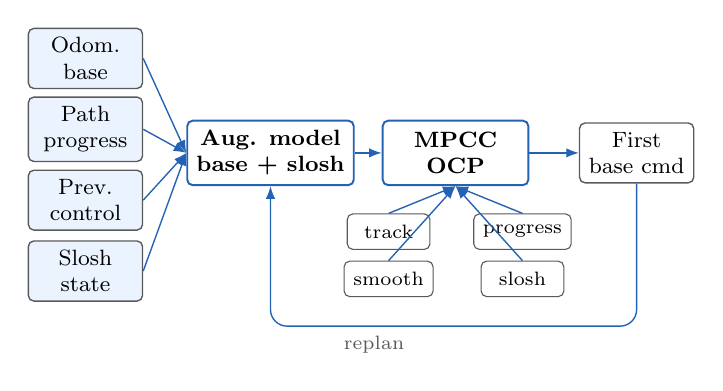
\begin{tikzpicture}[
    font=\footnotesize,
    block/.style={draw=spmpcgray, rounded corners=2pt, line width=0.5pt, fill=spmpclight, minimum width=1.45cm, minimum height=0.62cm, align=center},
    core/.style={draw=spmpcblue, rounded corners=2pt, line width=0.7pt, fill=white, minimum width=1.85cm, minimum height=0.82cm, align=center, font=\footnotesize\bfseries},
    cost/.style={draw=spmpcgray, rounded corners=2pt, line width=0.4pt, fill=white, minimum width=1.05cm, minimum height=0.45cm, align=center, font=\scriptsize},
    arr/.style={-{Latex[length=1.6mm]}, line width=0.5pt, draw=spmpcblue}
  ]
    \node[block] (odom) at (0,1.35) {Odom.\\base};
    \node[block] (path) at (0,0.45) {Path\\progress};
    \node[block] (prev) at (0,-0.45) {Prev.\\control};
    \node[block] (slosh) at (0,-1.35) {Slosh\\state};

    \node[core] (dyn) at (2.35,0.15) {Aug. model\\base + slosh};
    \node[core] (ocp) at (4.70,0.15) {\MPCC{}\\OCP};
    \node[block, fill=white] (cmd) at (7.00,0.15) {First\\base cmd};

    \node[cost] (c1) at (3.85,-0.85) {track};
    \node[cost] (c2) at (5.55,-0.85) {progress};
    \node[cost] (c3) at (3.85,-1.45) {smooth};
    \node[cost] (c4) at (5.55,-1.45) {slosh};

    \foreach \s in {odom,path,prev,slosh}
      \draw[arr] (\s.east) -- (dyn.west);
    \draw[arr] (dyn.east) -- (ocp.west);
    \draw[arr] (ocp.east) -- (cmd.west);
    \foreach \c in {c1,c2,c3,c4}
      \draw[arr] (\c.north) -- (ocp.south);
    \draw[arr, rounded corners=6pt] (cmd.south) |- (4.70,-2.05) -| node[pos=0.22, below, font=\scriptsize, text=spmpcgray] {replan} (dyn.south);
  \end{tikzpicture}}
  \caption{\SPMPC{} augmented-state and OCP structure. The planner puts the base state, path progress, and low-order slosh state in the same prediction model, jointly considers path tracking, path advancement, control smoothness, and predicted slosh response, and executes only the first base command.}
  \label{fig:method_structure}
\end{figure}

\subsection{Augmented State and Low-Order Slosh Dynamics}

To jointly represent path tracking and forward progress, we use an alpha-state \MPCC{} formulation with a path-progress variable.
The robot and progress state is
\begin{equation}
  \xr =
  \begin{bmatrix}
    p_x & p_y & \theta & v & s & \omega
  \end{bmatrix}^{\top},
\end{equation}
where $(p_x,p_y)$ is the base position, $\theta$ is the heading, $v$ is the linear velocity, $\omega$ is the angular velocity, and $s$ is the progress along the reference path.
The control input is
\begin{equation}
  \vu =
  \begin{bmatrix}
    a & \alpha & v_s
  \end{bmatrix}^{\top},
\end{equation}
where $a$ is the linear acceleration, $\alpha=\dot{\omega}$ is the angular acceleration, and $v_s=\dot{s}$ is the virtual path-progress speed.
The continuous-time robot model is
\begin{equation}
\begin{aligned}
  \dot{p}_x &= v\cos\theta, &
  \dot{p}_y &= v\sin\theta, &
  \dot{\theta} &= \omega, \\
  \dot{v} &= a, &
  \dot{s} &= v_s, &
  \dot{\omega} &= \alpha .
\end{aligned}
\label{eq:robot_alpha_dynamics}
\end{equation}
This state choice places base executability and path progress inside the same OCP: the planner cannot reduce sloshing simply by stopping, nor can it pursue progress while ignoring base constraints and liquid response.

Slosh-estimation studies under planar excitation show that dominant liquid response can be represented by a small number of modal coordinates and velocities excited by container acceleration \cite{A01_Leva2021}.
Model-based slosh estimation further shows that mass-spring-damper-type low-order models can provide control-oriented prediction quantities without high-fidelity free-surface computation \cite{A02_Guagliumi2021}.
Following this principle, we use a second-order modal model at the local-planning layer.
For each direction,
\begin{equation}
  x_{s,i}=
  \begin{bmatrix}
    \eta_i & \dot{\eta}_i
  \end{bmatrix}^{\top}, \qquad i\in\{x,y\},
\end{equation}
where $\eta_i$ and $\dot{\eta}_i$ are the displacement and velocity of the dominant slosh mode.
The dynamics are
\begin{equation}
  \ddot{\eta}_i
  +2\zeta_i\omega_i\dot{\eta}_i
  +\omega_i^2\eta_i
  =-\kappa_i a_i,
  \label{eq:slosh_modal_dynamics}
\end{equation}
where $\omega_i$, $\zeta_i$, and $\kappa_i$ are the equivalent natural frequency, damping ratio, and input gain, respectively, and $a_i$ is the horizontal excitation in the corresponding direction.

For planar motion of the wheeled base, the container excitation is approximated from the base motion:
\begin{equation}
  a_x = a, \qquad a_y \approx v\omega .
  \label{eq:slosh_excitation}
\end{equation}
Here $a_x$ denotes tangential excitation in the base-forward direction, and $a_y$ approximates lateral centripetal excitation during turning.
If inertial measurements or liquid-surface feedback are introduced in an extended implementation, this excitation channel can be replaced by measured or filtered container acceleration.
In this paper, it is used as a model-driven slosh-state propagation channel and is not treated as a real liquid-surface observer.

The two-direction liquid state is
\begin{equation}
  \xl =
  \begin{bmatrix}
    \eta_x & \dot{\eta}_x & \eta_y & \dot{\eta}_y
  \end{bmatrix}^{\top}.
\end{equation}
To distinguish internal planner quantities from measured liquid motion, we denote slosh-height quantities derived from the low-order state as $H_{\mathrm{model}}$.
We use two model proxies.
The first is a modal proxy based only on modal displacement:
\begin{equation}
  H_{\mathrm{model}}^{\mathrm{modal}}(t)
  = c_h\sqrt{\eta_x^2(t)+\eta_y^2(t)},
  \label{eq:h_model_modal}
\end{equation}
where $c_h$ maps modal displacement to an approximate height scale determined by container geometry, fill level, and modal parameters.
The second includes an optional quasi-static parabolic term during turning:
\begin{equation}
  H_{\mathrm{model}}^{\mathrm{full}}(t)
  = H_{\mathrm{model}}^{\mathrm{modal}}(t)
  + \mathbb{I}_{\mathrm{para}}\frac{R^2\omega^2(t)}{4g},
  \label{eq:h_model_full}
\end{equation}
where $R$ is the container radius, $\omega$ is the base angular velocity, and $\mathbb{I}_{\mathrm{para}}$ indicates whether the parabolic term is enabled.
Both $H_{\mathrm{model}}^{\mathrm{modal}}$ and $H_{\mathrm{model}}^{\mathrm{full}}$ are internal prediction or diagnostic proxies, not independent measurements of the real liquid surface.
This follows the evaluation discipline used in cross-platform anti-slosh trajectory planning, where low-order model height proxies are compared with video-extracted liquid motion \cite{C01_Ferrari2026}.

The augmented state is
\begin{equation}
\begin{aligned}
  \xaug = [&p_x,\ p_y,\ \theta,\ v,\ s,\ \omega, \\
           &\eta_x,\ \dot{\eta}_x,\ \eta_y,\ \dot{\eta}_y]^{\top}.
\end{aligned}
\label{eq:augmented_state}
\end{equation}
The augmented state is important not only because it supplies a slosh penalty to the objective, but because it makes liquid dynamic memory explicit in the prediction model.
If the state contained only base pose, velocity, and path progress, the future liquid response would still depend on unmodeled excitation history and the current liquid phase.
With $\eta_i$ and $\dot{\eta}_i$ included, the discrete prediction model becomes
\begin{equation}
  \xaug_{k+1}=f_d(\xaug_k,\vu_k),
\end{equation}
so the next augmented state is determined by the current augmented state and control input.
The slosh modal state is therefore part of the OCP state space, allowing the planner to predict how the current liquid phase will evolve under candidate future controls.

\subsection{Slosh-Aware MPCC Problem}

Let the reference path be
\begin{equation}
  \vr(s)=
  \begin{bmatrix}
    r_x(s) & r_y(s)
  \end{bmatrix}^{\top},
\end{equation}
with tangent angle $\psi(s)$.
The unit tangent and normal vectors are
\begin{equation}
\begin{aligned}
  \bm{t}(s) &= [\cos\psi(s),\ \sin\psi(s)]^{\top}, \\
  \bm{n}(s) &= [-\sin\psi(s),\ \cos\psi(s)]^{\top}.
\end{aligned}
\end{equation}
The position error relative to the path point is
\begin{equation}
  \bm{e}(s)=
  \begin{bmatrix}
    p_x & p_y
  \end{bmatrix}^{\top}-\vr(s).
\end{equation}
The contouring and lag errors are
\begin{equation}
  \ec = \bm{n}(s)^{\top}\bm{e}(s), \qquad
  \el = \bm{t}(s)^{\top}\bm{e}(s).
  \label{eq:contour_lag_error}
\end{equation}
The contouring error $\ec$ measures the lateral deviation from the reference path, and the lag error $\el$ measures the progress-direction deviation.
By optimizing $\ec$, $\el$, and $v_s$ jointly, \MPCC{} trades off path tracking and forward progress.

After discretizing \eqref{eq:robot_alpha_dynamics}--\eqref{eq:slosh_excitation}, let $N$ be the horizon length and $\Delta t$ be the time step.
At each control cycle, \SPMPC{} solves
\begin{equation}
\begin{aligned}
  \min_{\xaug_{0:N},\vu_{0:N-1}} \quad
  & \sum_{k=0}^{N-1}\ell_k + \ell_N \\
  \mathrm{s.t.}\quad
  & \xaug_0=\hat{\xaug}(t), \\
  & \xaug_{k+1}=f_d(\xaug_k,\vu_k), \\
  & \xaug_k\in\mathcal{X},\quad \vu_k\in\mathcal{U}, \\
  & k=0,\ldots,N-1 .
\end{aligned}
\label{eq:spmpc_ocp}
\end{equation}
Here $f_d$ is the discretized augmented dynamics and $\hat{\xaug}(t)$ is the current augmented-state estimate.
The stage and terminal costs are
\begin{equation}
\begin{aligned}
  \ell_k ={}& q_c e_{\mathrm{c},k}^{2}
    + q_l e_{\mathrm{l},k}^{2}
    - q_p v_{s,k}
    + q_v (v_k-v_{\mathrm{ref},k})^2 \\
  & + q_{v_s}(v_{s,k}-v_{\mathrm{ref},k})^2
    + \|\vu_k\|_{R}^{2} \\
  & + \|\vu_k-\vu_{k-1}\|_{S}^{2}
    + \|\bm{x}_{\ell,k}\|_{Q_s}^{2}, \\
  \ell_N ={}& q_{c,N}e_{\mathrm{c},N}^{2}
    + q_{l,N}e_{\mathrm{l},N}^{2}
    + \|\bm{x}_{\ell,N}\|_{Q_{s,N}}^{2} .
\end{aligned}
\label{eq:spmpc_cost_terms}
\end{equation}
The weights $q_c$ and $q_l$ penalize contouring and lag errors, $q_p$ rewards path progress, $q_v$ and $q_{v_s}$ make physical speed and virtual progress speed track the speed reference, $R$ penalizes control magnitude, $S$ penalizes control variation, and $Q_s$ penalizes predicted slosh state.
When the reference governor is disabled, $v_{\mathrm{ref},k}=v_{\mathrm{ref}}^{\mathrm{nom}}$.
When it is enabled, $v_{\mathrm{ref},k}=v_{\mathrm{ref}}^{g}$.

The key additional term in \eqref{eq:spmpc_cost_terms} is $\|\bm{x}_{\ell,k}\|_{Q_s}^{2}$, together with the corresponding slosh dynamics.
A planner that only increases control-smoothness penalties can prefer smooth command sequences, but it cannot distinguish two similarly smooth sequences that interact differently with the current residual slosh phase.
The augmented slosh state provides that distinction.

\begin{table}[t]
  \centering
  \scriptsize
  \setlength{\tabcolsep}{3pt}
  \caption{Roles of the \SPMPC{} objective terms.}
  \label{tab:cost_story}
  \begin{tabular}{p{0.25\linewidth} p{0.31\linewidth} p{0.32\linewidth}}
    \toprule
    Term & Optimization role & Functional interpretation \\
    \midrule
    $q_c\ec^2$, $q_l\el^2$ & Keep the base close to the reference path & Preserve local-planner path-tracking capability \\
    $-q_p v_s$ & Encourage progress along the path & Avoid reducing slosh simply by stopping \\
    $q_v(v-v_{\mathrm{ref}})^2$, $q_{v_s}(v_s-v_{\mathrm{ref}})^2$ & Track speed reference & Provide a common action point for nominal and governed references \\
    $\|\vu\|_R^2$ & Limit command magnitude & Maintain executable base commands \\
    $\|\Delta\vu\|_S^2$ & Smooth control variation & Limit changes in linear and angular commands \\
    $\|\xl\|_{Q_s}^2$ & Penalize predicted slosh state & Make predicted liquid response affect local motion selection \\
    \bottomrule
  \end{tabular}
\end{table}

The feasible sets mainly include base-motion constraints, control-input constraints, and path-progress constraints, for example
\begin{align}
  0 \leq v_k \leq v_{\max}, \qquad
  |\omega_k| \leq \omega_{\max}, \\
  |a_k| \leq a_{\max}, \qquad
  |\alpha_k| \leq \alpha_{\max}, \qquad
  0 \leq v_{s,k} \leq v_{s,\max} .
  \label{eq:spmpc_bounds}
\end{align}
These constraints ensure that the optimized trajectory can be converted to executable base commands.

The basic \SPMPC{} planner uses the slosh-state cost as the online anti-slosh mechanism.
If a model-predicted liquid boundary must be represented, the same augmented-state framework can include a soft boundary constraint such as
\begin{equation}
  \eta_{x,k}^{2}+\eta_{y,k}^{2} \leq \eta_{\max}^{2} + \epsilon_k,
  \qquad \epsilon_k\geq 0,
  \label{eq:slosh_soft_bound}
\end{equation}
with a slack penalty in the objective.
This extension is not treated as the core component of the physical experiments.
Moreover, \eqref{eq:slosh_soft_bound} is a model-predicted boundary; without real liquid-surface feedback and a formal safety proof, it is not a spill-free guarantee.

\subsection{Slosh-risk Reference Governor}

The \MPCC{} formulation above selects local motion inside the OCP through the augmented state and slosh cost.
To further regulate task speed when short-horizon prediction indicates elevated slosh risk, we introduce a soft Slosh-risk Reference Governor.
The module is placed before the \MPCC{} solve.
Its only role is to contract the nominal speed reference $v_{\mathrm{ref}}^{\mathrm{nom}}$ into a governed reference $v_{\mathrm{ref}}^{g}$, which then enters \eqref{eq:spmpc_cost_terms}.
It does not directly modify the solved base command, does not act as an emergency brake or hard safety interlock, does not use RGB liquid observations, and does not change the \MPCC{} state dimension.

Given the current slosh state $\xl(t)$, base speed $v(t)$, angular speed $\omega(t)$, and nominal speed reference $v_{\mathrm{ref}}^{\mathrm{nom}}$, the governor searches over a finite set of scaling factors
\begin{equation}
  \mathcal{B}
  =\{\beta_0,\ldots,\beta_{M-1}\}
  \subseteq[\beta_{\min},1].
  \label{eq:governor_beta_grid}
\end{equation}
Each candidate $\beta$ defines
\begin{equation}
  v_{\beta}=\beta v_{\mathrm{ref}}^{\mathrm{nom}},
\end{equation}
and is evaluated by an internal $N_g$-step rollout.
In the implementation, the predicted speed $v_k^g$ approaches $v_{\beta}$ under a prescribed acceleration limit, the angular velocity can be approximated by time-constant decay, and the slosh state is propagated using the low-order model in \eqref{eq:slosh_modal_dynamics}--\eqref{eq:slosh_excitation}.
Let $H_k(\beta)\geq 0$ be the model-predicted slosh height or envelope proxy at step $k$ for candidate $\beta$, using either $H_{\mathrm{model}}^{\mathrm{modal}}$ or $H_{\mathrm{model}}^{\mathrm{full}}$ according to the evaluation convention.
With a normalization height $H_{\lim}>0$, the candidate risk is
\begin{equation}
  R(\beta)
  =
  \max_{0\leq k\leq N_g}
  \frac{H_k(\beta)}{H_{\lim}} .
  \label{eq:governor_candidate_risk}
\end{equation}
For a risk threshold $\rho$, the feasible candidate set is
\begin{equation}
  \mathcal{B}_{\mathrm{feas}}
  =
  \{\beta\in\mathcal{B}\mid R(\beta)\leq \rho\}.
  \label{eq:governor_beta_feas}
\end{equation}
The raw scaling factor is selected as
\begin{equation}
  \beta_{\mathrm{raw}}
  =
  \begin{cases}
    \max \mathcal{B}_{\mathrm{feas}}, & \mathcal{B}_{\mathrm{feas}}\neq \emptyset,\\
    \beta_{\min}, & \mathcal{B}_{\mathrm{feas}}= \emptyset.
  \end{cases}
  \label{eq:governor_beta_star}
\end{equation}
If $\mathcal{B}_{\mathrm{feas}}$ is empty, the state is marked as saturated.
This status indicates that every discrete candidate exceeds the model-predicted risk threshold, so the system uses the smallest candidate reference for soft deceleration.
It is not a formal safety stop condition.

To avoid abrupt speed-reference changes, the governor applies an asymmetric rate limit to $\beta_{\mathrm{raw}}$.
Let $\beta_f^{-}$ be the filtered scaling factor from the previous cycle, and let $\dot{\beta}_{\uparrow}$ and $\dot{\beta}_{\downarrow}$ be the increase and decrease rate limits.
Then
\begin{equation}
  \begin{aligned}
    \underline{\beta}
    &=\max\{\beta_{\min},\beta_f^{-}-\dot{\beta}_{\downarrow}\Delta t\},\\
    \overline{\beta}
    &=\min\{1,\beta_f^{-}+\dot{\beta}_{\uparrow}\Delta t\},\\
    \beta_f
    &=\operatorname{clip}
      \left(\beta_{\mathrm{raw}},\underline{\beta},\overline{\beta}\right).
  \end{aligned}
  \label{eq:governor_beta_filter}
\end{equation}
The governed reference sent to the \MPCC{} problem is
\begin{equation}
  \tilde{v}_{\mathrm{ref}}^{g}
  =
  \beta_f v_{\mathrm{ref}}^{\mathrm{nom}},
  \qquad
  v_{\mathrm{ref}}^{g}
  =
  \min\left\{
    v_{\mathrm{ref}}^{\mathrm{nom}},
    \max\{v_{\min},\tilde{v}_{\mathrm{ref}}^{g}\}
  \right\}.
  \label{eq:governor_vref}
\end{equation}
When no minimum cruising speed is used, \eqref{eq:governor_vref} reduces to $v_{\mathrm{ref}}^{g}=\beta_f v_{\mathrm{ref}}^{\mathrm{nom}}$.
Because $v_{\mathrm{ref}}^{g}$ only enters the speed-reference terms of the \MPCC{} problem, the final base command is still determined by the \MPCC{} solution, base constraints, and execution interface.

\noindent\textbf{Proposition 1 (reference non-amplification and discrete candidate optimality).}
Assume $v_{\mathrm{ref}}^{\mathrm{nom}}\geq 0$, $H_{\lim}>0$, $\mathcal{B}\subseteq[\beta_{\min},1]$, and the filtered scaling factor in \eqref{eq:governor_beta_filter} satisfies $\beta_f\in[\beta_{\min},1]$.
Then the governor satisfies $v_{\mathrm{ref}}^{g}\leq v_{\mathrm{ref}}^{\mathrm{nom}}$.
If $\mathcal{B}_{\mathrm{feas}}$ is nonempty, then $\beta_{\mathrm{raw}}$ is the largest scaling factor in the discrete candidate set that satisfies the model-predicted risk threshold.

\noindent\emph{Proof.}
From \eqref{eq:governor_beta_filter}, $\beta_f\leq 1$, and therefore $\tilde{v}_{\mathrm{ref}}^{g}=\beta_f v_{\mathrm{ref}}^{\mathrm{nom}}\leq v_{\mathrm{ref}}^{\mathrm{nom}}$.
Equation \eqref{eq:governor_vref} then explicitly applies $\min\{v_{\mathrm{ref}}^{\mathrm{nom}},\cdot\}$, giving $v_{\mathrm{ref}}^{g}\leq v_{\mathrm{ref}}^{\mathrm{nom}}$.
Furthermore, \eqref{eq:governor_beta_feas}--\eqref{eq:governor_beta_star} selects the maximum element among all discrete candidates satisfying $R(\beta)\leq\rho$.
Thus, when the feasible set is nonempty, $\beta_{\mathrm{raw}}$ is the maximum feasible scaling factor on the candidate grid.

The above property is not a spill-free or safety-invariance guarantee.
If the rate limiter yields $\beta_f>\beta_{\mathrm{raw}}$, then a rollout at $\beta_f$ may still exceed the risk threshold; this condition is reported as a transient rate-limited state rather than a satisfied safety constraint.
If no candidate satisfies the threshold, the governor enters the saturated state and takes $\beta_{\min}$, which remains a soft reference-adaptation action rather than a hard stop or formal safety controller.

\subsection{Receding-Horizon Execution and Ablation Variants}

After solving \eqref{eq:spmpc_ocp}, the planner executes only the first optimized step.
The command sent to the base can be obtained from the first predicted state or from the current velocity plus the optimized control increment, for example
\begin{equation}
  v_{\mathrm{cmd}} = v_0 + a_0^{\star}\Delta t,
  \qquad
  \omega_{\mathrm{cmd}} = \omega_0 + \alpha_0^{\star}\Delta t.
  \label{eq:cmd_generation}
\end{equation}
The command is then passed through the base-interface limits and published as the base velocity command.
At the next cycle, the system reinitializes with updated odometry and the updated model slosh state and solves again.
This receding-horizon execution preserves the interface of an ordinary mobile-robot local planner.

The method supports modular ablations.
To test whether smooth motion alone explains anti-slosh behavior, the experiments use four variants within the same \MPCC{} framework, as shown in \cref{tab:method_variants}.

\begin{table}[t]
  \centering
  \scriptsize
  \setlength{\tabcolsep}{3pt}
  \caption{\SPMPC{} internal ablation variants.}
  \label{tab:method_variants}
  \begin{tabular}{p{0.18\linewidth} p{0.22\linewidth} p{0.20\linewidth} p{0.28\linewidth}}
    \toprule
    Variant & Slosh model/cost & Smoothing & Experimental question \\
    \midrule
    \Bzero{} & absent & weak & Can the base \MPCC{} complete path tracking? \\
    \Bsmooth{} & absent & strong & Is stronger control smoothing sufficient? \\
    \Bslosh{} & present & weak & Does explicit slosh-state prediction have independent value? \\
    \Bours{} & present & strong & How does the state-augmented planner trade tracking, smoothness, and slosh response? \\
    \bottomrule
  \end{tabular}
\end{table}

The comparison between \Bsmooth{} and \Bslosh{} separates control smoothness from liquid-state prediction.
\Bours{} denotes the basic \SPMPC{} planner.
When the reference-adaptation module is evaluated, it is enabled on top of the same \Bours{} parameters and nominal speed reference and is denoted \Boursgov{}.
This isolates the incremental effect of soft speed-reference adaptation relative to the basic slosh-state-augmented \MPCC{}.

\section{Experiments and Validation}

The experiments evaluate the main claim of \SPMPC{}: explicit slosh-state prediction can provide interpretable liquid-response improvement beyond smooth-only control, without unacceptable path-tracking, task-time, or online-computation cost.
The evaluation uses a two-layer evidence chain.
Controlled comparisons are used to separate internal ablation factors and local-planner baselines, while physical trials examine external liquid response and the interpretability of internal model proxies.
Online computation and execution diagnostics are treated separately to verify that the method remains a deployable receding-horizon local planner.

\subsection{Experimental Setting and Metrics}

The experimental scope matches the problem formulation: a standard wheeled mobile base transports an open liquid container along a precomputed geometrically feasible reference path.
Planner comparisons use the same start and goal conditions, reference path, base constraints, task termination condition, and failure criteria.
External baseline planners do not receive liquid-surface state as a control input.
Each trial logs trajectory, velocity commands, control inputs, solve time, internal model proxies, and external liquid observations.
Throughout the evaluation, $H_{\mathrm{model}}^{\mathrm{modal}}$ and $H_{\mathrm{model}}^{\mathrm{full}}$ are interpreted only as internal prediction or diagnostic proxies.
Claims about real liquid motion are based on RGB envelope measurements, liquid-level measurements, or other external observations.

\begin{figure}[t]
  \centering
  \resizebox{\linewidth}{!}{%
  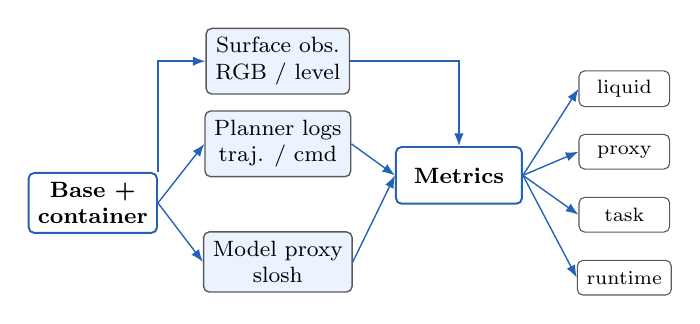
\begin{tikzpicture}[
    font=\footnotesize,
    block/.style={draw=spmpcgray, rounded corners=2pt, line width=0.5pt, fill=spmpclight, minimum width=1.55cm, minimum height=0.58cm, align=center},
    core/.style={draw=spmpcblue, rounded corners=2pt, line width=0.7pt, fill=white, minimum width=1.60cm, minimum height=0.72cm, align=center, font=\footnotesize\bfseries},
    metric/.style={draw=spmpcgray, rounded corners=2pt, line width=0.4pt, fill=white, minimum width=1.15cm, minimum height=0.44cm, align=center, font=\scriptsize},
    arr/.style={-{Latex[length=1.6mm]}, line width=0.5pt, draw=spmpcblue}
  ]
    \node[core] (robot) at (0,0) {Base +\\container};
    \node[block] (planner) at (2.35,0.75) {Planner logs\\traj. / cmd};
    \node[block] (proxy) at (2.35,-0.75) {Model proxy\\slosh};
    \node[block] (camera) at (2.35,1.80) {Surface obs.\\RGB / level};
    \node[core] (eval) at (4.65,0.35) {Metrics};
    \node[metric] (m1) at (6.75,1.45) {liquid};
    \node[metric] (m2) at (6.75,0.65) {proxy};
    \node[metric] (m3) at (6.75,-0.15) {task};
    \node[metric] (m4) at (6.75,-0.95) {runtime};

    \draw[arr] (robot.east) -- (planner.west);
    \draw[arr] (robot.east) -- (proxy.west);
    \draw[arr] (robot.north east) |- (camera.west);
    \draw[arr] (planner.east) -- (eval.west);
    \draw[arr] (proxy.east) -- (eval.west);
    \draw[arr] (camera.east) -| (eval.north);
    \foreach \m in {m1,m2,m3,m4}
      \draw[arr] (eval.east) -- (\m.west);
  \end{tikzpicture}}
  \caption{Experimental measurement pipeline. Trajectories, base commands, solve time, and internal slosh proxies explain planner behavior; real liquid-response claims are supported by external vision or liquid-level observations.}
  \label{fig:experiment_setup}
\end{figure}

\Cref{tab:metrics_plan} summarizes the metrics.
For liquid-response comparisons, high-percentile and RMS metrics are emphasized because single-frame maxima can be affected by isolated visual envelope spikes.
For limited sample sizes, the statistical claim is restricted to representative evidence rather than broad population-level significance.

\begin{table}[t]
  \centering
  \scriptsize
  \setlength{\tabcolsep}{3pt}
  \caption{Evaluation metrics and their roles.}
  \label{tab:metrics_plan}
  \begin{tabular}{p{0.27\linewidth} p{0.35\linewidth} p{0.26\linewidth}}
    \toprule
    Category & Metrics & Purpose \\
    \midrule
    External liquid motion & RGB max-LCR, RMS-LCR, residual oscillation & Test whether external observations support liquid-response improvement \\
    Model diagnostics & Predicted slosh state, $H_{\mathrm{model}}^{\mathrm{modal}}$, $H_{\mathrm{model}}^{\mathrm{full}}$ & Interpret model prediction without replacing external measurements \\
    Model-external consistency & $\gamma_{\mathrm{bias}}$, $\gamma_{\mathrm{abs}}$, RMSE, $\rho$, $\tau^\star$, peak/high-percentile underestimation & Check whether internal proxies explain external observations \\
    Task completion & Success rate, timeout, arrival time & Exclude the explanation that the planner simply stops or slows excessively \\
    Path tracking & Contouring error, path deviation & Verify that the local-planning task remains satisfied \\
    Control smoothness & RMS velocity, acceleration, and angular acceleration & Separate smoothness from slosh-state prediction \\
    Online computation & Solve time, control frequency, solver failures & Verify real-time receding-horizon execution \\
    \bottomrule
  \end{tabular}
\end{table}

To avoid evaluating the method using only internal model quantities, we compare model proxies with an external liquid observation $H_{\mathrm{vis}}(t)$.
Let $H_{\mathrm{model}}^{\mathrm{eval}}(t)$ denote the model proxy used for comparison; it may be either $H_{\mathrm{model}}^{\mathrm{modal}}(t)$ or $H_{\mathrm{model}}^{\mathrm{full}}(t)$, and the selected convention is reported with the results.
Following the practice of comparing low-order model height with video-extracted liquid motion in anti-slosh trajectory planning \cite{C01_Ferrari2026}, we define the signed bias
\begin{equation}
  \gamma_{\mathrm{bias}} =
  100\cdot
  \frac{\int_{t_0}^{t_1}\left(H_{\mathrm{model}}^{\mathrm{eval}}(t)-H_{\mathrm{vis}}(t)\right)\dd t}
  {\int_{t_0}^{t_1}H_{\mathrm{model}}^{\mathrm{eval}}(t)\dd t+\epsilon}.
  \label{eq:gamma_bias}
\end{equation}
The interval $[t_0,t_1]$ spans the valid command window and the post-arrival residual-oscillation window, and $\epsilon$ prevents denominator degeneracy.
A positive $\gamma_{\mathrm{bias}}$ indicates that the model is conservative on average, while a negative value indicates average underestimation of the external metric.
The absolute deviation is
\begin{equation}
  \gamma_{\mathrm{abs}} =
  100\cdot
  \frac{\int_{t_0}^{t_1}\left|H_{\mathrm{model}}^{\mathrm{eval}}(t)-H_{\mathrm{vis}}(t)\right|\dd t}
  {\int_{t_0}^{t_1}H_{\mathrm{vis}}(t)\dd t+\epsilon}.
  \label{eq:gamma_abs}
\end{equation}
Additional diagnostics include RMSE, correlation coefficient $\rho$, phase shift $\tau^\star$, peak error, high-percentile error, and maximum local underestimation.
Model-external consistency is used for interpretation; it is not a substitute for external liquid evidence and does not constitute a formal spill-prevention guarantee.

\subsection{Internal Ablation and Baseline Structure}

The internal ablation tests whether \SPMPC{} is merely a stronger smoothness controller.
All variants share the same path-progress \MPCC{} structure, reference path, and base constraints; they differ only in the slosh model/cost and smoothing weights.
The four variants \Bzero{}, \Bsmooth{}, \Bslosh{}, and \Bours{} are defined in \cref{tab:method_variants}.

\begin{figure}[t]
  \centering
  \resizebox{\linewidth}{!}{%
  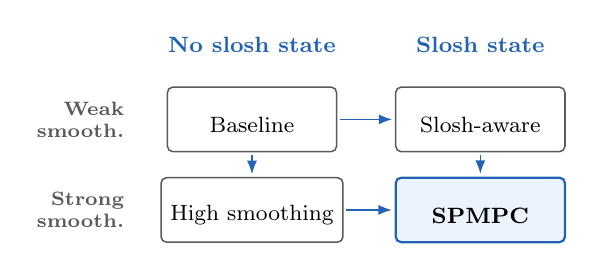
\begin{tikzpicture}[
    font=\footnotesize,
    cell/.style={draw=spmpcgray, rounded corners=2pt, line width=0.55pt, fill=white, minimum width=2.15cm, minimum height=0.82cm, align=center},
    ours/.style={draw=spmpcblue, rounded corners=2pt, line width=0.8pt, fill=spmpclight, minimum width=2.15cm, minimum height=0.82cm, align=center, font=\footnotesize\bfseries},
    head/.style={font=\footnotesize\bfseries, text=spmpcblue, align=center},
    row/.style={font=\scriptsize\bfseries, text=spmpcgray, align=right},
    arr/.style={-{Latex[length=1.7mm]}, line width=0.5pt, draw=spmpcblue, shorten >=1pt, shorten <=1pt}
  ]
    \node[head] at (1.45,1.65) {No slosh state};
    \node[head] at (4.35,1.65) {Slosh state};
    \node[row, anchor=east] at (-0.05,0.70) {Weak\\smooth.};
    \node[row, anchor=east] at (-0.05,-0.45) {Strong\\smooth.};

    \node[cell] (b0) at (1.45,0.70) {\Bzero{}\\Baseline};
    \node[cell] (bs) at (4.35,0.70) {\Bslosh{}\\Slosh-aware};
    \node[cell] (bm) at (1.45,-0.45) {\Bsmooth{}\\High smoothing};
    \node[ours] (bo) at (4.35,-0.45) {\Bours{}\\SPMPC};

    \draw[arr] (b0) -- (bs);
    \draw[arr] (b0) -- (bm);
    \draw[arr] (bm) -- (bo);
    \draw[arr] (bs) -- (bo);
  \end{tikzpicture}}
  \caption{Internal ablation structure. The variants form a two-factor decomposition of whether the planner propagates a slosh state and whether stronger control smoothing is applied.}
  \label{fig:ablation_design}
\end{figure}

The comparisons answer distinct questions.
\Bsmooth{} vs.\ \Bzero{} quantifies the effect of stronger smoothness alone.
\Bslosh{} vs.\ \Bzero{} evaluates the independent role of explicit slosh-state prediction.
\Bours{} vs.\ \Bsmooth{} tests whether the state-augmented planner exceeds smooth-only planning.
\Bours{} vs.\ \Bslosh{} characterizes the role of additional smoothing in executable local-command generation.
Only trends supported by external liquid observations are interpreted as real liquid-response improvement; reductions in internal proxies alone are interpreted as model-side reductions in predicted slosh response.

Ordinary local-planner baselines test whether online local planning without liquid-state propagation already covers the task.
Candidate baselines include DWA, TEB, \MpcLocalPlanner{}, and LT-DWA.
They operate at a similar deployment layer and generate executable base commands, but generally do not propagate liquid dynamic memory.
Quantitative comparison requires runnable interfaces, matched base constraints, identical task definitions, and reproducible logs.
Mobile-base anti-slosh reference methods, such as Hamaguchi-style path/speed profiles, input shaping, and offline liquid-constrained trajectory optimization, are included quantitatively only when they can be reproduced under comparable platform and interface conditions; otherwise, they serve as decision-layer references rather than ranked baselines.

The Slosh-risk Reference Governor is evaluated as an incremental module by comparing \Bours{} and \Boursgov{} under the same \SPMPC{} parameters, nominal speed reference, and base constraints.
In addition to liquid, task, and tracking metrics, the governor-specific diagnostics are $\beta_{\mathrm{raw}}$, $\beta_f$, saturated rate, transient rate-limited rate, and arrival-time change.

\subsection{Physical Experiments: External Liquid Response and Model Consistency}

Physical experiments examine whether the trends observed from planning and model proxies are supported by external liquid-surface observations.
The platform records the final base command, external liquid observation, internal model proxy, and execution-chain diagnostics, allowing the analysis to separate planner behavior from base execution, sensing latency, and command limiting.
In the physical analysis, $H_{\mathrm{model}}$ remains an internal proxy; real liquid-response conclusions are based on RGB or liquid-level observations.

\Cref{tab:real_fixed_path_ablation} reports a representative fixed-path internal-ablation result.
The comparison includes a basic baseline, a smooth-only baseline, and a slosh-aware variant.
Each method is repeated three times.
All trials reach the goal, and the valid configurations use $v_{\mathrm{ref}}=0.20\,\mathrm{m/s}$, matched linear/angular velocity and acceleration limits, enabled fixed closed-loop delay compensation, disabled hard model constraint, and no tracking-protection stop.
Statistics are computed over the 10--90\% path-progress window.

\begin{table}[t]
  \centering
  \scriptsize
  \setlength{\tabcolsep}{3pt}
  \renewcommand{\arraystretch}{1.05}
  \caption{Representative fixed-path physical internal-ablation results over the 10--90\% path-progress window.}
  \label{tab:real_fixed_path_ablation}
  \label{tab:real_reduction_selected}
  \resizebox{\columnwidth}{!}{%
  \begin{tabular}{lccc}
    \toprule
    Metric & \Bzero{} & \Bsmooth{} & \Bslosh{} \\
    \midrule
    \multicolumn{4}{l}{\textit{A. Physical ablation statistics}}\\
    Model p95 [mm] & $1.100\pm0.034$ & $0.994\pm0.165$ & $0.632\pm0.101$ \\
    Model max [mm] & $2.102\pm0.222$ & $2.227\pm0.240$ & $1.255\pm0.039$ \\
    Model RMS [mm] & $0.547\pm0.016$ & $0.491\pm0.066$ & $0.307\pm0.035$ \\
    RGB p95 [mm] & $1.009\pm0.214$ & $1.272\pm0.283$ & $0.901\pm0.015$ \\
    RGB max [mm] & $2.398\pm0.482$ & $2.267\pm0.309$ & $2.162\pm0.405$ \\
    RGB RMS [mm] & $0.541\pm0.081$ & $0.639\pm0.060$ & $0.537\pm0.008$ \\
    Projection p95 [cm] & $2.947\pm0.087$ & $3.646\pm1.188$ & $3.442\pm0.128$ \\
    $|\omega|$ p95 [rad/s] & $0.234\pm0.015$ & $0.202\pm0.022$ & $0.242\pm0.033$ \\
    Arrival time [s] & $33.753\pm0.355$ & $35.169\pm0.537$ & $36.851\pm0.231$ \\
    \midrule
    \multicolumn{4}{l}{\textit{B. Relative reduction of \Bslosh{} with respect to \Bsmooth{}}}\\
    Model p95 & -- & -- & $36.4\%$ \\
    Model RMS & -- & -- & $37.4\%$ \\
    RGB p95 & -- & -- & $29.2\%$ \\
    RGB RMS & -- & -- & $15.9\%$ \\
    \bottomrule
  \end{tabular}}
\end{table}

The comparison between \Bsmooth{} and \Bzero{} shows that stronger smoothing can reduce $|\omega|$ p95 and some model-proxy statistics, but the RGB liquid envelope does not decrease accordingly.
\Bslosh{} does not have the lowest $|\omega|$ p95, yet both the model-proxy and RGB p95/RMS metrics are lower than those of \Bsmooth{}.
This indicates that the observed liquid-response improvement in these representative trials cannot be explained by smaller angular velocity alone.
Panel B of \cref{tab:real_fixed_path_ablation} reports the corresponding relative reductions.

Relative to the smooth-only baseline, \Bslosh{} reduces the model-proxy p95 and RMS by 36.4\% and 37.4\%, and reduces the RGB $H_{\mathrm{vis}}$ p95 and RMS by 29.2\% and 15.9\%.
Peak statistics are retained in \cref{tab:real_fixed_path_ablation}, but the isolated sensitivity of max values to visual envelope spikes makes p95/RMS the primary evidence in this comparison.
Relative to \Bzero{}, \Bslosh{} reduces the model proxy and RGB p95, while the RGB RMS is nearly unchanged; therefore \Bzero{} is used as a reference baseline rather than the main reduction denominator.
Overall, these representative fixed-path physical trials show consistent p95/RMS liquid-response improvement of the slosh-aware variant over the smooth-only baseline.
At the same time, \Bslosh{} has a longer arrival time, and its projection-error and angular-velocity statistics are not uniformly best.
The conclusion is therefore limited to liquid-response improvement rather than dominance across all task metrics.

The model-external comparison is used only as an interpretive diagnostic.
In this result, the internal model proxy $H_{\mathrm{model}}$ and the external RGB liquid envelope decrease consistently when comparing \Bslosh{} against \Bsmooth{}, supporting a trend-level explanation based on explicit slosh prediction.
The proxy still cannot replace external liquid observations, frame-level phase fidelity, ground-truth free-surface height, or hard safety monitoring.

\subsection{Online Computation and Execution Diagnostics}

Online solve performance is reported separately from liquid-response metrics to verify that \SPMPC{} remains a deployable receding-horizon local planner rather than an offline anti-slosh trajectory optimizer.
Relevant quantities include OCP solve-time distribution, control frequency, solver failures, timeouts, and extreme cases.
Median and high-percentile solve times are compared with the control period.

Execution diagnostics explain discrepancies in the physical system.
They include optimizer output, final base velocity command, command saturation, terminal deceleration, sensing delay, and base response.
These diagnostics support experimental interpretation but are not independent anti-slosh contributions.
When the execution chain substantially modifies the optimizer output, the corresponding physical conclusions are interpreted under that execution condition.

% \section{Conclusion and Limitations}

This paper studied online local planning for mobile-base open-liquid transport and proposed \SPMPC{}, a slosh-aware planning method that embeds low-order slosh modal states into an \MPCC{} formulation.
The central premise is that liquid sloshing is not only a trajectory-smoothing issue, but a state-prediction problem with dynamic memory.
If a planner penalizes only velocity, acceleration, or command variation, it may fail to represent the effect of the current liquid phase on future response.
\SPMPC{} forms an augmented state from base motion, path progress, and low-order slosh variables, jointly optimizes contouring error, lag error, path progress, control magnitude, control smoothness, and predicted slosh response, and executes the first optimized base command in receding horizon.
The paper also formulates a soft Slosh-risk Reference Governor as a pre-\MPCC{} finite-horizon reference-adaptation module that contracts the speed reference without directly rewriting the final base command.

Representative fixed-path physical trials provide initial evidence for the main claim.
For \Bzero{}, \Bsmooth{}, and \Bslosh{}, three trials per method reached the goal.
Over the 10--90\% path-progress window, \Bslosh{} reduced the model-proxy p95 and RMS by 36.4\% and 37.4\% relative to the smooth-only baseline, and reduced RGB $H_{\mathrm{vis}}$ p95 and RMS by 29.2\% and 15.9\%.
These p95/RMS trends indicate that the slosh-aware variant can provide liquid-response improvement beyond smooth-only control in the representative trials.
The evidence is deliberately interpreted conservatively: RGB RMS decreases less than the model proxy, \Bslosh{} takes longer to reach the goal, and its path-projection and angular-velocity metrics are not uniformly best.
Internal model proxies are therefore treated as control-side diagnostic quantities rather than ground-truth liquid height, complete candidate-ranking criteria, or hard safety signals.

The conclusions hold under the assumptions of a precomputed geometrically feasible reference path, low-order slosh modeling, and external liquid-response evaluation.
\SPMPC{} is positioned as a method for moving liquid dynamic memory into the online \MPCC{} local-planning layer of a standard mobile base, not as a high-fidelity free-surface reconstruction method or a formal spill-free controller.
The Slosh-risk Reference Governor is likewise a soft reference-adaptation mechanism, not a hard safety interlock or a spill-prevention proof.
Future extensions include broader validation across paths, fill levels, container geometries, ordinary local-planner baselines, mobile-base anti-slosh references, and governor ablations, as well as measured container acceleration, real liquid-surface feedback, and uncertainty-aware constraints for more complex navigation scenarios.


\bibliographystyle{IEEEtran}
\bibliography{references}

\end{document}
